\section*{Problem Setting and Goals}
\label{sec:setting}
%%%%%%%%%%%%%%%%%%%%%%%%%%%%%%%%%%%%%%%%%%%%%%%%%%%%%%%%%%%%%%%%%%%%%


The paper considers a dataset $\bm{x} \!\in\! \cX \subseteq \RR^k$ of $n$ entities,
whose elements $x_i= (x_{i1},\ldots, x_{1k})$ describe $k$ measurable
quantities of entity $i \!\in\! [n]$, such as the number of individuals living
in a geographical region $i$ and their English proficiency.
The paper considers two classes of problems:
\begin{itemize}[leftmargin=*,labelsep=2pt,itemsep=0pt,parsep=2pt,topsep=2pt]
	\item An \emph{allotment problem} $P : \cX \times [n] \to \mathbb{R}$ is a function that distributes a finite set of resources to some problem entity. $P$ may represent, for instance, the amount of money allotted to a school district.
	\item A \emph{decision rule} $P: \cX \times [n] \to \{0,1\}$
	determines whether some entity qualifies for some benefits. For
	instance, $P$ may represent if election ballots should be described
	in a minority language for an electoral district.
% https://www.justice.gov/crt/about-language-minority-voting-rights
\end{itemize}
The paper assumes that $P$ has bounded range, and uses the shorthand
$P_i(\bm{x})$ to denote $P(\bm{x}, i)$ for entity $i$.
%
The focus of the paper is to study the effects of a DP data-release
mechanism $\cM$ to the outcomes of problem $P$. Mechanism $\cM$ is
applied to the dataset $\bm{x}$ to produce a privacy-preserving
counterpart $\tilde{\bm{x}}$ and the resulting private outcome
$P_i(\tilde{\bm{x}})$ is used to make some allocation decisions.

\begin{figure}[!t]
	\centering
	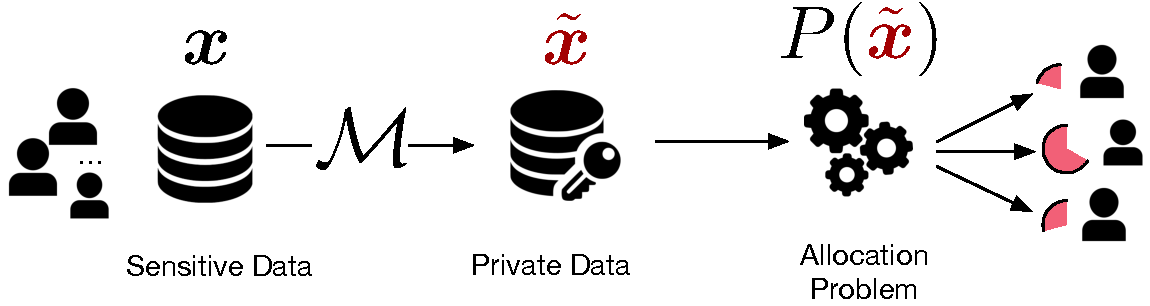
\includegraphics[width=0.9\columnwidth]{images/figure.pdf}
	\caption{Diagram of the private allocation problem.}
	\label{fig:framework}
\end{figure}
Figure \ref{fig:framework} provides an illustrative diagram.

Because random noise is added to the original dataset $\bm{x}$, the output $P_i(\tilde{\bm{x}})$ incurs some error. {\em The focus of this paper is to characterize and quantify the disparate impact of this error among the problem entities}. In particular, the paper focuses on two notations of errors.

\begin{definition}[Statistical bias]
	\label{def:bias}
	The statistical bias  $ B_P^i(\cM, \bm{x}) $ of the mechanism $\cM$ measures the difference between the expected private outcome with the true outcome:
	\begin{equation}
		\label{eq:bias}
		B_P^i(\cM, \bm{x}) =
		%\left|
		\EE_{\tilde{\bm{x}} \sim \cM(\bm{x})} \left[ P_i(\tilde{\bm{x}}) \right] - P_i (\bm{x}),
		%\right|,
	\end{equation}

\end{definition}

The paper also considers another notation of error which is the normalized version of the above bias.
\begin{definition}[Multiplicative error]
	The multiplicative error under mechanism $\cM$ and problem $P$ for entity $i$ is given by: $\nicefrac{B_P^i(\cM, \bm{x})}{P^i(x)}$

\end{definition}

Our notion of fairness will be based on these two notations of errors.

\begin{definition}[$\alpha$-fairness \cite{fioretto:CP-19}]
	Given the true data $\truedata$, the mechanism $\cM$ is said to be \emph{$\alpha$-fair} if, for any $i\in[n]$,
	\begin{equation*}
		\xi^{i}_P(\cM, \bm{x}) = ~\left\vert  B_P^i(\cM, \bm{x}) - B_P^j(\cM, \bm{x})
		\right\vert\leq \alpha\,,
	\end{equation*}
	where $ \xi^{i}_P(\cM, \bm{x})$ is referred to as the \emph{disparity error} associated with
	district $i$. The mechanism $\cM$ is \emph{$\alpha'$-minimally fair} if $\alpha'=\inf \alpha$ such that
	$\cM$ is $\alpha$-fair. To put it differently, the mechanism $\cM$ is \emph{$\alpha'$-minimally fair} if
	\begin{align*}
		\alpha'& = \max_{j\neq i}~\left\vert  B_P^i(\cM, \bm{x}) - B_P^j(\cM, \bm{x})
		\right\vert \\
		&= \max_{j\in [n]} B_P^j(\cM, \bm{x})   -\min_{j\in [n]}~ B_P^j(\cM, \bm{x}) \,.
	\end{align*}
\end{definition}
Throughout this report, every time we say that a mechanism is $\alpha$-fair, we mean that
it is $\alpha$-minimally fair.

% which characterizes the distance between the expected
% privacy-preserving allocation and the one based on the ground truth.
% The paper considers the absolute bias $|B_P^i|$, in place of the bias
% $B_P^i$, when $P$ is a decision rule. The distinction will become
% clear in the next sections.

%%%%%%%%%%%%%%%%%%%%%%%%%%%%%%%%%%%%%%%%%%%%%%%%%%%%%%%%%%%%%%%%%%%%%
